\chapter{Lower Bounds for Sorting, Dual-Pivot Quicksort, and Bounded Quicksort}
\label{cha:lecture-four}

\begin{center}
  \textbf{Lecture 4}\\
  \emph{Lower Bounds (RAM vs Two-Level Model), Dual-Pivot Quicksort, and Bounded Quicksort}\\[0.5em]
  Date: September 28, 2026
\end{center}

This chapter investigates the theoretical and engineering analysis of complexity lower bounds for the fundamental problem of comparison-based sorting, contrasting the classical RAM model with the two-level memory model of Aggarwal and Vitter. Subsequently, the focus shifts to modern architectural developments of the \textit{Quicksort} algorithm: we analyze the duplicate keys problem and the \textit{Dual-Pivot Quicksort} algorithm introduced by Yaroslavskiy, followed by a formal treatment of the \textit{Bounded Quicksort} (BQS) variant. We rigorously prove how tail recursion elimination and bounded partitioning guarantee an auxiliary stack space strictly bounded by $\Theta(\log_2 n)$, while achieving optimal cache efficiency via an \textit{Insertion Sort} cutoff.

\FloatBarrier
\section{RAM Model: Lower Bounds and Decision Trees}
\label{sec:ram-lower-bounds}

In the standard RAM (\textit{Random Access Machine}) model of computation, a comparison-based algorithm cannot inspect the underlying bitwise representation of keys to extract digits or radix components (as done in \textit{Radix Sort} algorithms). Instead, it may only acquire information regarding the relative ordering of elements via binary comparisons of the form:
\begin{equation}
  A < B, \quad A = B, \quad \text{or} \quad A > B.
\end{equation}
Assuming, without loss of generality for lower bound derivations, that all input keys are pairwise distinct, each elementary comparison yields a strictly dichotomous outcome ($<$ or $>$).

\subsection{The Decision Tree Model}
\label{subsec:decision-tree-model}

The family of deterministic comparison-based algorithms is formally modeled through the abstract mathematical structure of a \textbf{Decision Tree}:

\begin{itemize}
  \item \textbf{Internal nodes:} Each internal node models a single elementary comparison between a pair of input elements or positions, conventionally denoted by $[A : B]$. Since all keys are distinct, exactly two directed edges leave the node, corresponding to the two mutually exclusive outcomes: the left edge associated with $A < B$ and the right edge with $A > B$. Consequently, the decision tree is a proper binary tree.
  \item \textbf{Root-to-leaf path:} For any given input instance of size $n$, the deterministic algorithm traces a unique directed path from the root down to a leaf. Each node visited along this trajectory corresponds to a comparison executed by the algorithm; the length of the path (the number of traversed edges) reflects the exact comparison count for that specific configuration. The length of the longest root-to-leaf path corresponds to the \textbf{height} $t$ of the decision tree and quantifies the worst-case running time $T(n)$.
  \item \textbf{Leaves:} Each leaf corresponds to algorithmic termination and encapsulates the final solution or output configuration of the computational problem (e.g., the permutation of indices that sorts the array, or the index at which the target key is located).
\end{itemize}

\autoref{fig:decision-tree-model} illustrates the general topological structure of a binary decision tree for a generic comparison-based problem.

\begin{figure}[H]
  \centering
  \begin{tikzpicture}[
    scale=0.92,
    node distance=1.5cm,
    cmp/.style={rectangle, draw=blue!75!black, fill=blue!8, thick, rounded corners=3pt, minimum width=1.9cm, minimum height=0.65cm, font=\small\bfseries, align=center},
    leaf/.style={rectangle, draw=green!60!black, fill=green!12, thick, rounded corners=3pt, minimum width=1.0cm, minimum height=0.62cm, font=\small\bfseries, align=center},
    edgeLbl/.style={font=\scriptsize\bfseries, fill=white, inner sep=1.5pt},
    arr/.style={-{Stealth[scale=1.0]}, thick, draw=blue!80!black}
  ]
    % Root
    \node[cmp] (root) at (0, 0) {$A : B$};
    
    % Level 1
    \node[cmp] (L1) at (-2.8, -1.4) {$C : D$};
    \node[cmp] (R1) at (2.8, -1.4) {$E : F$};
    
    \draw[arr] (root) -- node[edgeLbl, above left] {$A < B$} (L1);
    \draw[arr] (root) -- node[edgeLbl, above right] {$A > B$} (R1);
    
    % Level 2
    \node[cmp] (LL2) at (-4.4, -2.8) {$G : H$};
    \node[cmp] (LR2) at (-1.6, -2.8) {$I : J$};
    \node[cmp] (RL2) at (1.6, -2.8) {$K : L$};
    \node[cmp] (RR2) at (4.4, -2.8) {$M : N$};
    
    \draw[arr] (L1) -- node[edgeLbl, left] {$<$} (LL2);
    \draw[arr] (L1) -- node[edgeLbl, right] {$>$} (LR2);
    \draw[arr] (R1) -- node[edgeLbl, left] {$<$} (RL2);
    \draw[arr] (R1) -- node[edgeLbl, right] {$>$} (RR2);
    
    % Ellipses for intermediate depth
    \node at (-4.4, -3.6) {$\vdots$};
    \node at (-1.6, -3.6) {$\vdots$};
    \node at (1.6, -3.6) {$\vdots$};
    \node at (4.4, -3.6) {$\vdots$};
    
    % Distinct terminal leaves (problem solutions)
    \node[leaf] (leaf1) at (-5.1, -4.7) {$S_1$};
    \node[leaf] (leaf2) at (-3.7, -4.7) {$S_2$};
    \node[leaf] (leaf3) at (-1.6, -4.7) {$S_3$};
    \node[font=\small\bfseries, text=gray!80!black] (leafmid1) at (0.0, -4.7) {$\dots$};
    \node[leaf] (leafk) at (1.6, -4.7) {$S_k$};
    \node[font=\small\bfseries, text=gray!80!black] (leafmid2) at (2.65, -4.7) {$\dots$};
    \node[leaf] (leafn1) at (3.7, -4.7) {$S_{n-1}$};
    \node[leaf] (leafn) at (5.1, -4.7) {$S(n)$};
    
    \draw[arr, dashed] (-4.4, -3.9) -- (leaf1);
    \draw[arr, dashed] (-4.4, -3.9) -- (leaf2);
    \draw[arr, dashed] (-1.6, -3.9) -- (leaf3);
    \draw[arr, dashed] (1.6, -3.9) -- (leafk);
    \draw[arr, dashed] (4.4, -3.9) -- (leafn1);
    \draw[arr, dashed] (4.4, -3.9) -- (leafn);
    
    % Height quota t
    \draw[{Stealth[scale=1.1]}-{Stealth[scale=1.1]}, thick, draw=red!70!black] (6.0, 0) -- (6.0, -4.7) 
      node[midway, right=4pt, align=left, font=\footnotesize\bfseries, text=red!80!black] {Height $t$\\ $\ge \log_2 S(n)$};
    \draw[draw=gray!50, dashed] (root.east) -- (6.1, 0);
    \draw[draw=gray!50, dashed] (leafn.east) -- (6.1, -4.7);
    
    % Bottom brace for leaf count
    \draw[decorate, decoration={brace, amplitude=6pt, mirror}, thick, draw=green!60!black] (-5.7, -5.2) -- (5.7, -5.2)
      node[midway, below=7pt, font=\small\bfseries, text=green!50!black] {Leaves (distinct solutions): total count $\le 2^t$, with $2^t \ge S(n)$};
  \end{tikzpicture}
  \caption{Binary decision tree model for comparison-based algorithms. Internal nodes represent elementary pairwise comparisons; leaves represent admissible distinct solutions ($S_1, S_2, \dots, S(n)$). The longest path determines the worst-case running time.}
  \label{fig:decision-tree-model}
\end{figure}

\subsection{The General Information-Theoretic Lower Bound}
\label{subsec:general-information-theorem}

The fundamental relationship between the number of distinct solutions of a problem and the minimum number of comparisons necessary to solve it is established by the following information-theoretic theorem.

\begin{theorem}[General Information-Theoretic Lower Bound]
\label{thm:information-theoretic-bound}
Let $P$ be a computational problem solvable via a deterministic comparison-based algorithm. If for an input of size $n$ the problem admits $S(n)$ distinct possible solutions (each of which must be returned by the algorithm for suitable input configurations), then any deterministic comparison-based algorithm requires in the worst case:
\begin{equation}
  T(n) = \Omega(\log_2 S(n)).
\end{equation}
\end{theorem}

\begin{proof}
Consider the binary decision tree associated with an arbitrary correct deterministic algorithm for problem $P$. Let $t$ denote the height of the tree, representing the maximum length of any root-to-leaf path.

Because comparisons are strictly binary (assuming distinct keys), every internal node has at most $2$ children. By induction on height, a binary tree of height $t$ possesses at most $L$ leaves, bounded by:
\begin{equation}
  L \le 2^t.
\end{equation}
For the algorithm to be correct on every valid input instance, the decision tree must be capable of reaching each of the $S(n)$ distinct solutions. Consequently, each distinct solution must be associated with at least one distinct leaf in the tree (if two distinct solutions mapped to the same leaf, the algorithm would fail to discriminate between them, outputting an erroneous answer for at least one of the instances). Hence, we must have:
\begin{equation}
  2^t \ge L \ge S(n).
\end{equation}
Applying the base-$2$ logarithm (a strictly monotonically increasing function) to both sides yields:
\begin{equation}
  t \ge \log_2 S(n).
\end{equation}
Since the worst-case time complexity $T(n)$ is defined as the height $t$ of the tree, we conclude that:
\begin{equation}
  T(n) \ge \log_2 S(n) \implies T(n) = \Omega(\log_2 S(n)).
\end{equation}
\end{proof}

\subsection{Fundamental Applications: Searching and Sorting}
\label{subsec:search-and-sort-applications}

\autoref{thm:information-theoretic-bound} directly yields canonical lower bounds for two core computational problems in internal memory:

\begin{enumerate}
  \item \textbf{Searching a Key (\textit{Searching}):}
  Given a sorted array of $n$ elements and a target key $K$, the algorithm must determine whether $K$ resides in the array and, if so, return its index $i \in \{1, 2, \dots, n\}$; if absent, it returns an explicit failure symbol $\bot$. The set of distinct valid outputs is:
  \begin{equation}
    S(n) = \{1, 2, \dots, n\} \cup \{\bot\} \implies |S(n)| = n + 1.
  \end{equation}
  Applying the theorem:
  \begin{equation}
    T_{\text{Search}}(n) \ge \log_2(n + 1) = \Omega(\log_2 n).
  \end{equation}
  This lower bound establishes the asymptotic optimality of \textit{Binary Search}, which operates in exactly $\Theta(\log_2 n)$ comparisons.

  \item \textbf{Sorting (\textit{Sorting}):}
  Given an array of $n$ distinct elements, sorting is equivalent to identifying which of the $n!$ permutations of indices rearranges the keys in non-decreasing order. Since the set $\{1, 2, \dots, n\}$ admits exactly $n!$ distinct permutations, the number of possible solutions is:
  \begin{equation}
    S(n) = n!.
  \end{equation}
  Applying the lower bound theorem:
  \begin{equation}
    T_{\text{Sort}}(n) \ge \log_2(n!).
  \end{equation}
  To express this bound in explicit asymptotic form, we invoke \textbf{Stirling's approximation} for the factorial:
  \begin{equation}
    n! \approx \sqrt{2\pi n} \left(\frac{n}{e}\right)^n \implies \ln(n!) = n \ln n - n + \mathcal{O}(\ln n).
  \end{equation}
  Converting to base-$2$ logarithm:
  \begin{equation}
    \log_2(n!) = n \log_2 n - n \log_2 e + \Theta(\log_2 n) = \Theta(n \log_2 n).
  \end{equation}
  Alternatively, using an elementary lower bound over the upper half of terms:
  \begin{align}
    n! &\ge \prod_{i = \lceil n/2 \rceil}^{n} i \ge \left(\frac{n}{2}\right)^{n/2}, \\
    \log_2(n!) &\ge \frac{n}{2} \log_2\left(\frac{n}{2}\right) = \frac{n}{2}(\log_2 n - 1) = \Omega(n \log_2 n).
  \end{align}
  Therefore:
  \begin{equation}
    T_{\text{Sort}}(n) = \Omega(n \log_2 n).
  \end{equation}
  Any deterministic or randomized comparison-based sorting algorithm (such as \textit{Merge Sort}, \textit{Heap Sort}, or the expected time of \textit{Quicksort}) cannot surpass the asymptotic barrier $\Omega(n \log_2 n)$ in the RAM model.
\end{enumerate}

\FloatBarrier
\section{Two-Level Memory: Aggarwal-Vitter Lower Bound}
\label{sec:aggarwal-vitter-lower-bound}

In the two-level memory model introduced by Aggarwal and Vitter~\cite{aggarwal1988}, the primary computational cost is not measured by elementary CPU comparisons, but by the total number $t$ of I/O operations, each transferring a contiguous block of $B$ elements between slow external storage and internal RAM of capacity $M$ items.

\subsection{The Nature of I/O and Free In-Memory Comparisons}
\label{subsec:free-comparisons-intuition}

The standard binary decision tree cannot be directly applied to external memory analysis:
\begin{itemize}
  \item A single disk read operation simultaneously brings an entire block of $B$ elements into fast internal memory.
  \item Once these $B$ elements reside in RAM alongside the remaining $M - B$ elements already present, the CPU can execute \textbf{an arbitrary number of in-memory comparisons at zero I/O cost}.
  \item These "free" internal comparisons permit sorting all $M$ items currently in RAM, drastically pruning the set of candidate global permutations consistent with the current knowledge.
\end{itemize}

Consequently, to establish an external memory lower bound, one must formulate an \textbf{I/O Decision Tree}, where each node represents an I/O read operation (loading a block of size $B$), and outgoing edges correspond to all possible relative arrangements resulting from interleaving the $B$ retrieved elements with the $M - B$ elements already residing in RAM.

\subsection{Branching Factor (Fan-out) Calculation of the I/O Tree}
\label{subsec:fanout-calculation}

When a block of $B$ elements is transferred from disk into internal memory (accommodating $M$ elements total, consisting of $M - B$ pre-existing elements and $B$ newly loaded items), we distinguish two operational scenarios:

\begin{enumerate}
  \item \textbf{Reading a "New Block" (\textit{New Block}):}
  The block is transferred from disk for the very first time: its elements have never been observed before by any previous step of the algorithm.
  \begin{itemize}
    \item The mutual relative order of the $B$ elements is completely unknown: they can appear in any of the $B!$ possible permutations.
    \item Once placed in RAM, the $B$ new items must be interleaved with the $M - B$ pre-existing items to establish their combined sorted order within the $M$ slots. The number of ways to interleave $B$ elements into $M$ positions is given by the binomial coefficient:
    \begin{equation}
      \binom{M}{B} = \frac{M!}{B! \, (M - B)!}.
    \end{equation}
  \end{itemize}
  Multiplying the $B!$ internal ordering possibilities by the $\binom{M}{B}$ interleaving positions, the branching factor (\textit{fan-out}) $X$ for reading a new block is:
  \begin{equation}
    X = (B!) \cdot \binom{M}{B}.
    \label{eq:fanout-new-block}
  \end{equation}

  \item \textbf{Re-reading an "Old Block" (\textit{Old Block}):}
  The block was previously read, internally sorted, and written back to disk during an earlier phase of computation (such as an intermediate run generated during multiway merging).
  \begin{itemize}
    \item The internal relative order among its $B$ elements is already fully known; hence, no new information is acquired regarding their intrinsic ordering (a factor of $1$ rather than $B!$).
    \item The only new information gained is how these $B$ elements interleave with the other $M - B$ items currently in RAM.
  \end{itemize}
  The branching factor (\textit{fan-out}) $Y$ for re-reading an old block is therefore:
  \begin{equation}
    Y = \binom{M}{B}.
    \label{eq:fanout-old-block}
  \end{equation}
\end{enumerate}

\autoref{fig:io-decision-tree} summarizes the logical dichotomy and branch cardinalities for both I/O transfer types.

\begin{figure}[H]
  \centering
  \begin{tikzpicture}[
    scale=0.95,
    box/.style={rectangle, draw=blue!80!black, fill=blue!8, thick, rounded corners=4pt, minimum width=4.2cm, minimum height=1.0cm, align=center, font=\small\bfseries},
    branch/.style={rectangle, draw=orange!80!black, fill=orange!8, thick, rounded corners=3pt, minimum width=5.5cm, minimum height=2.2cm, align=left, font=\footnotesize},
    arr/.style={-{Stealth[scale=1.1]}, thick, draw=blue!70!black}
  ]
    % Top I/O node
    \node[box] (ioNode) at (0, 2.7) {I/O Read Operation\\(Loads $B$ elements into memory $M$)};
    
    % Left Branch: New Block
    \node[branch] (newBlock) at (-3.8, -0.8) {
      \textbf{\textcolor{orange!90!black}{A) New Block (\textit{New Block})}}\\[3pt]
      $\bullet$ $B$ elements never seen before;\\
      $\bullet$ $B!$ possible internal permutations;\\
      $\bullet$ $\binom{M}{B}$ ways to interleave into $M$ slots;\\[4pt]
      \textbf{Branching factor (Fan-out):}\\[2pt]
      \null\hfill $X = (B!) \cdot \binom{M}{B}$\hfill\null
    };
    
    % Right Branch: Old Block
    \node[branch] (oldBlock) at (3.8, -0.8) {
      \textbf{\textcolor{orange!90!black}{B) Old Block (\textit{Old Block})}}\\[3pt]
      $\bullet$ Block already processed previously;\\
      $\bullet$ Internal order among $B$ elements already known;\\
      $\bullet$ $\binom{M}{B}$ ways to interleave into $M$ slots;\\[4pt]
      \textbf{Branching factor (Fan-out):}\\[2pt]
      \null\hfill $Y = \binom{M}{B}$\hfill\null
    };
    
    \draw[arr] (ioNode.south) -- ++(0, -0.5) -| node[pos=0.25, above=2pt, font=\scriptsize\bfseries] {First read} (newBlock.north);
    \draw[arr] (ioNode.south) -- ++(0, -0.5) -| node[pos=0.25, above=2pt, font=\scriptsize\bfseries] {Subsequent re-read} (oldBlock.north);
  \end{tikzpicture}
  \caption{Branching factors (\textit{fan-out}) in the I/O decision tree under the two-level memory model: reading a new block yields internal order information ($B!$) and interleaving information ($\binom{M}{B}$); re-reading an old block yields only interleaving information.}
  \label{fig:io-decision-tree}
\end{figure}

\subsection{Formal Derivation of the Aggarwal-Vitter Lower Bound}
\label{subsec:formal-derivation-av}

Consider an input file consisting of $n$ distinct elements stored across $N = \frac{n}{B}$ disk blocks. In order to sort the file, any correct algorithm must inspect each element at least once; consequently, it must execute at least $\frac{n}{B}$ "New Block" read operations.

If the algorithm executes a total of $t$ I/O operations in the worst case, then:
\begin{itemize}
  \item Exactly $\frac{n}{B}$ operations will be of type "New Block", each with fan-out at most $X$.
  \item The remaining $t - \frac{n}{B}$ operations will be (at most) of type "Old Block", each with fan-out at most $Y$.
\end{itemize}

The total number of leaves in the I/O decision tree represents the maximum number of global permutations distinguishable by this sequence of transfers. For the algorithm to correctly sort any valid instance, this leaf count must be at least equal to $n!$:
\begin{equation}
  X^{\frac{n}{B}} \cdot Y^{\left(t - \frac{n}{B}\right)} \ge n!.
  \label{eq:io-tree-leaves-inequality}
\end{equation}

Substituting the explicit formulas for $X$ and $Y$ from equations~(\ref{eq:fanout-new-block}) and~(\ref{eq:fanout-old-block}):
\begin{equation}
  \left[ (B!) \cdot \binom{M}{B} \right]^{\frac{n}{B}} \cdot \left[ \binom{M}{B} \right]^{t - \frac{n}{B}} \ge n!.
\end{equation}
Collecting powers sharing the common base $\binom{M}{B}$:
\begin{equation}
  (B!)^{\frac{n}{B}} \cdot \binom{M}{B}^{\frac{n}{B}} \cdot \binom{M}{B}^{t - \frac{n}{B}} \ge n! \implies (B!)^{\frac{n}{B}} \cdot \binom{M}{B}^t \ge n!.
  \label{eq:leaves-compact-inequality}
\end{equation}

Taking the base-$2$ logarithm on both sides of inequality~(\ref{eq:leaves-compact-inequality}):
\begin{equation}
  \log_2\left((B!)^{\frac{n}{B}}\right) + \log_2\left(\binom{M}{B}^t\right) \ge \log_2(n!),
\end{equation}
which yields:
\begin{equation}
  \frac{n}{B} \log_2(B!) + t \log_2\binom{M}{B} \ge \log_2(n!).
  \label{eq:log-leaves-inequality}
\end{equation}

To expand the logarithmic expressions, we use standard asymptotic bounds for the factorial and the binomial coefficient:
\begin{itemize}
  \item By Stirling's approximation: $\log_2(a!) \approx a \log_2 a - a \log_2 e \approx a \log_2 a$.
  \item For the binomial coefficient, recalling that $\binom{a}{b} \le \left(\frac{e \cdot a}{b}\right)^b$:
  \begin{equation}
    \log_2 \binom{M}{B} \approx B \log_2\left(\frac{M}{B}\right) + \mathcal{O}(B).
  \end{equation}
\end{itemize}

Substituting these expressions into equation~(\ref{eq:log-leaves-inequality}):
\begin{equation}
  \frac{n}{B} \cdot \left(B \log_2 B\right) + t \cdot \left(B \log_2 \frac{M}{B}\right) \ge n \log_2 n.
\end{equation}
Simplifying the factor $B$ in the first term:
\begin{equation}
  n \log_2 B + t \cdot B \log_2\left(\frac{M}{B}\right) \ge n \log_2 n.
\end{equation}

Isolating the term containing the unknown $t$:
\begin{equation}
  t \cdot B \log_2\left(\frac{M}{B}\right) \ge n \log_2 n - n \log_2 B = n \left(\log_2 n - \log_2 B\right) = n \log_2\left(\frac{n}{B}\right).
\end{equation}
Dividing both sides by the strictly positive quantity $B \log_2\left(\frac{M}{B}\right)$:
\begin{equation}
  t \ge \frac{n \log_2\left(\frac{n}{B}\right)}{B \log_2\left(\frac{M}{B}\right)} = \frac{n}{B} \cdot \frac{\log_2(n / B)}{\log_2(M / B)}.
\end{equation}

Applying the change of base formula for logarithms ($\frac{\log_2 a}{\log_2 b} = \log_b a$), we formally obtain the renowned Aggarwal-Vitter lower bound theorem.

\begin{theorem}[Aggarwal-Vitter Lower Bound for External Sorting]
\label{thm:aggarwal-vitter-bound}
Under the two-level memory model, any deterministic or randomized comparison-based sorting algorithm requires in the worst case:
\begin{equation}
  \text{I/O}_{\text{Sort}}(n) = \Omega\left(\frac{n}{B} \log_{M/B}\left(\frac{n}{B}\right)\right) = \Omega\left(\frac{n}{B} \frac{\log(n / B)}{\log(M / B)}\right) \text{ I/Os}.
\end{equation}
\end{theorem}

\begin{property}[Asymptotic Optimality of Multiway Merge Sort]
The Aggarwal-Vitter lower bound demonstrates that the \textbf{Multiway Merge Sort} ($k$-Way Merge Sort with merge degree $k = \frac{M}{B} - 1$) analyzed in Lecture~\ref{cha:lecture-three} (\autoref{sec:multiway-merge-sort}) is \textbf{asymptotically optimal}: the total number of I/O operations required to sort the array matches the fundamental theoretical lower bound dictated by information theory in external memory.
\end{property}

\FloatBarrier
\section{Quicksort: Duplicate Handling and Dual-Pivot Quicksort}
\label{sec:quicksort-and-dual-pivot}

\textit{Quicksort} is a \textit{Divide and Conquer} algorithm based on distribution (\textit{distribution-based}): rather than rigidly partitioning the array by index positions (as in \textit{Merge Sort}) and then merging the sorted subproblems, Quicksort partitions the data based on the relative magnitude of one or more privileged keys termed \textbf{pivots}, delegating all sorting work to the partitioning phase.

\subsection{The Equal Values Problem}
\label{subsec:equal-values-problem}

In traditional textbook implementations of Quicksort employing standard two-way partitioning (\textit{2-way partitioning}, such as Lomuto or Hoare schemes):
\begin{itemize}
  \item The array is divided into two parts: elements $\le p$ on one side and elements $> p$ on the other.
  \item Whenever the array contains many identical keys equal to pivot $p$ (in the extreme case, an array containing only identical keys, $S[i] = c, \forall i$), such a scheme places all duplicates into the same partition.
  \item As a consequence, the subproblem shrinks by only a single element per recursive call ($1$ versus $n-1$), collapsing the recursion tree into a degenerate chain of height $\Theta(n)$ and the overall running time to quadratic complexity:
  \begin{equation}
    T(n) = T(n - 1) + \Theta(n) = \Theta(n^2).
  \end{equation}
\end{itemize}

\begin{definition}[Three-Way Partitioning (Dutch National Flag)]
The classical remedy for duplicate keys, formulated by Edsger Dijkstra~\cite{dijkstra1976} as the Dutch National Flag problem, partitions the array into \textbf{three contiguous regions}:
\begin{equation}
  [\, < p \quad \mid \quad = p \quad \mid \quad > p \,].
\end{equation}
Elements strictly equal to the pivot ($= p$) are already in their final sorted positions and are \textbf{excluded from further recursive invocations}, which are executed solely on the $[< p]$ and $[> p]$ subranges. On arrays with all equal keys, this achieves linear running time $\mathcal{O}(n)$.
\end{definition}

\subsection{3-Way Partitioning Algorithm and Numerical Execution Example}
\label{subsec:3way-quicksort-example}

To practically implement three-way partitioning (\textit{Dutch National Flag}) in Quicksort, the linear-time algorithm designed by Dijkstra and formalized by Sedgewick~\cite{sedgewick1978} is widely adopted.

Given a sub-array $S[\text{lo} \dots \text{hi}]$ with the first element chosen as the pivot $p = S[\text{lo}]$, the algorithm maintains three operational indices during sequential scanning:
\begin{itemize}
  \item \textbf{Pointer $lt$ (\textit{less than}):} delimits elements strictly smaller than the pivot on the left. The invariant guarantees that $S[k] < p$ for all $\text{lo} \le k < lt$. Initially, $lt = \text{lo}$.
  \item \textbf{Pointer $i$ (scan cursor):} scans the array elements. The invariant ensures that $S[k] = p$ for all $lt \le k < i$. Initially, $i = \text{lo} + 1$.
  \item \textbf{Pointer $gt$ (\textit{greater than}):} delimits elements strictly greater than the pivot on the right. The invariant guarantees that $S[k] > p$ for all $gt < k \le \text{hi}$. Initially, $gt = \text{hi}$.
  \item The sub-array $S[i \dots gt]$ contains elements that have not yet been examined.
\end{itemize}

At each iteration, as long as $i \le gt$, the current element $S[i]$ is compared with the pivot $p$:
\begin{enumerate}
  \item \textbf{If $S[i] < p$:} swap $S[lt]$ and $S[i]$, then increment both indices ($lt \leftarrow lt + 1$, $i \leftarrow i + 1$). Because by invariant cell $S[lt]$ held an element equal to $p$, swapping moves the smaller element to the left and places a pivot duplicate at $S[i]$, allowing $i$ to advance.
  \item \textbf{If $S[i] > p$:} swap $S[i]$ and $S[gt]$, then decrement only $gt$ ($gt \leftarrow gt - 1$). The index $i$ \textbf{does not advance}, because the element just swapped from $S[gt]$ has not yet been compared.
  \item \textbf{If $S[i] == p$:} the element is already in the correct central region; increment only the scan cursor ($i \leftarrow i + 1$).
\end{enumerate}

Upon termination ($i > gt$), the array is partitioned into three distinct contiguous regions: $S[\text{lo} \dots lt-1] < p$, $S[lt \dots gt] = p$, and $S[gt+1 \dots \text{hi}] > p$. Subsequent recursive calls are issued \textbf{exclusively} on $S[\text{lo} \dots lt-1]$ and $S[gt+1 \dots \text{hi}]$, bypassing the entire duplicate block. The formal dimensional invariants of these partitions and their integration with the order statistics selection algorithm (\textit{Quickselect}) and expected-time recurrence relation are explored in depth in Lecture~\ref{cha:lecture-five} (\autoref{sec:3way-partitioning}).

\autoref{tab:3way-execution-trace} details the step-by-step progress of the three pointers and array contents throughout the execution with pivot $p = 4$.

\begin{table}[H]
  \centering
  \small
  \begin{tabularx}{\textwidth}{c c c c >{\centering\arraybackslash}p{2.6cm} >{\raggedright\arraybackslash}X >{\centering\arraybackslash}p{3.2cm}}
    \toprule
    \textbf{Step} & $\boldsymbol{i}$ & $\boldsymbol{lt}$ & $\boldsymbol{gt}$ & \textbf{Comparison} & \textbf{Action} & \textbf{Array State} \\
    \midrule
    Init & 1 & 0 & 7 & Pivot $p = 4$ & Initialization & $[4, 7, 2, 4, 1, 4, 8, 3]$ \\
    1 & 1 & 0 & 7 & $S[1]=7 > 4$ & $\text{SWAP}(S[1], S[7])$, $gt \leftarrow 6$ & $[4, 3, 2, 4, 1, 4, 8, 7]$ \\
    2 & 1 & 0 & 6 & $S[1]=3 < 4$ & $\text{SWAP}(S[0], S[1])$, $lt \leftarrow 1$, $i \leftarrow 2$ & $[3, 4, 2, 4, 1, 4, 8, 7]$ \\
    3 & 2 & 1 & 6 & $S[2]=2 < 4$ & $\text{SWAP}(S[1], S[2])$, $lt \leftarrow 2$, $i \leftarrow 3$ & $[3, 2, 4, 4, 1, 4, 8, 7]$ \\
    4 & 3 & 2 & 6 & $S[3] == 4$ & Advance $i \leftarrow 4$ & $[3, 2, 4, 4, 1, 4, 8, 7]$ \\
    5 & 4 & 2 & 6 & $S[4]=1 < 4$ & $\text{SWAP}(S[2], S[4])$, $lt \leftarrow 3$, $i \leftarrow 5$ & $[3, 2, 1, 4, 4, 4, 8, 7]$ \\
    6 & 5 & 3 & 6 & $S[5] == 4$ & Advance $i \leftarrow 6$ & $[3, 2, 1, 4, 4, 4, 8, 7]$ \\
    7 & 6 & 3 & 6 & $S[6]=8 > 4$ & $\text{SWAP}(S[6], S[6])$, $gt \leftarrow 5$ & $[3, 2, 1, 4, 4, 4, 8, 7]$ \\
    \midrule
    \textbf{End} & \textbf{6} & \textbf{3} & \textbf{5} & $i > gt$ & \textbf{Termination} & $\mathbf{[3, 2, 1 \mid 4, 4, 4 \mid 8, 7]}$ \\
    \bottomrule
  \end{tabularx}
  \caption{Detailed step-by-step trace of 3-way partitioning with pivot $p = 4$. At termination, the three identical keys equal to $4$ occupy indices $lt \dots gt$ ($3 \dots 5$) and are bypassed by subsequent recursive calls.}
  \label{tab:3way-execution-trace}
\end{table}

\FloatBarrier

\subsection{Architecture of Dual-Pivot Quicksort (Yaroslavskiy)}
\label{subsec:dual-pivot-architecture}

In 2009, Russian engineer Vladimir Yaroslavskiy proposed an innovative algorithm called \textbf{Dual-Pivot Quicksort}~\cite{yaroslavskiy2009}. Following extensive empirical benchmarks conducted in collaboration with Joshua Bloch and Robert Sedgewick, the algorithm replaced classic single-pivot Quicksort in Java's standard library (`java.util.Arrays.sort`) for all primitive data types.

Unlike classical Quicksort, Dual-Pivot Quicksort chooses \textbf{two pivots} $P$ and $Q$. It first ensures $P \le Q$ (swapping them if necessary). The active subarray range $S[\text{left} \dots \text{right}]$ is dynamically divided into four regions managed via three operational indices ($l, k, g$):

\begin{itemize}
  \item $l$ (\textit{less}): upper bound of elements strictly smaller than $P$ ($S[i] < P$ for all $\text{left} \le i < l$).
  \item $k$: current scanning pointer ($l \le k \le g$). Elements between $l$ and $k-1$ satisfy the central invariant: $P \le S[i] \le Q$.
  \item $g$ (\textit{great}): lower bound of elements strictly greater than $Q$ ($S[i] > Q$ for all $g < i \le \text{right}$).
  \item The region between $k$ and $g$ holds items not yet examined.
\end{itemize}

\autoref{fig:dual-pivot-partition} illustrates the array layout during the execution of dual-pivot partitioning.

\begin{figure}[H]
  \centering
  \begin{tikzpicture}[
    scale=0.95,
    box/.style={draw, thick, minimum height=1.1cm, align=center, font=\small},
    ptr/.style={-{Stealth[scale=1.1]}, very thick, draw=blue!85!black},
    ptrLbl/.style={font=\small\bfseries, text=blue!90!black}
  ]
    % Array regions
    \node[box, fill=teal!18, minimum width=2.6cm] (r1) at (1.3, 0) {$S[i] < P$};
    \node[box, fill=orange!18, minimum width=3.8cm] (r2) at (4.5, 0) {$P \le S[i] \le Q$};
    \node[box, fill=gray!15, dashed, minimum width=3.2cm] (r3) at (8.0, 0) {Unexamined\\($k \dots g$)};
    \node[box, fill=purple!18, minimum width=2.6cm] (r4) at (10.9, 0) {$S[i] > Q$};
    
    % Array border
    \draw[thick] (0, -0.55) rectangle (12.2, 0.55);
    
    % Range bounds
    \node[left=5pt, font=\small\bfseries, text=black!75] at (0, 0) {$\text{left}$};
    \node[right=5pt, font=\small\bfseries, text=black!75] at (12.2, 0) {$\text{right}$};
    
    % Pointer arrows
    \draw[ptr] (2.6, -1.3) -- (2.6, -0.65);
    \node[below=2pt, ptrLbl] at (2.6, -1.3) {Pointer $l$};
    
    \draw[ptr] (6.4, -1.3) -- (6.4, -0.65);
    \node[below=2pt, ptrLbl] at (6.4, -1.3) {Pointer $k$};
    
    \draw[ptr] (9.6, -1.3) -- (9.6, -0.65);
    \node[below=2pt, ptrLbl] at (9.6, -1.3) {Pointer $g$};
    
    % Descriptive labels
    \node[above=6pt, font=\footnotesize\bfseries, text=teal!80!black] at (1.3, 0.55) {Smaller than $P$};
    \node[above=6pt, font=\footnotesize\bfseries, text=orange!85!black] at (4.5, 0.55) {Range $[P, Q]$};
    \node[above=6pt, font=\footnotesize\bfseries, text=gray!80!black] at (8.0, 0.55) {Unexamined};
    \node[above=6pt, font=\footnotesize\bfseries, text=purple!80!black] at (10.9, 0.55) {Greater than $Q$};
  \end{tikzpicture}
  \caption{Dual-Pivot Quicksort partitioning schema (Yaroslavskiy). The array is partitioned into four dynamic regions: elements $< P$, elements between $P$ and $Q$, unexamined elements between $k$ and $g$, and elements $> Q$.}
  \label{fig:dual-pivot-partition}
\end{figure}

\subsection{Invariants and Transition Logic}
\label{subsec:dual-pivot-invariants}

The partitioning procedure maintains the invariant until pointer $k$ crosses $g$ ($k \le g$). At each step, the element $S[k]$ is evaluated:

\begin{enumerate}
  \item \textbf{Case 1: $S[k] < P$:}
  The element belongs to the leftmost partition. It is swapped with $S[l]$, and both pointers are incremented:
  \begin{equation}
    \text{SWAP}(S[k], S[l]), \quad l \leftarrow l + 1, \quad k \leftarrow k + 1.
  \end{equation}
  Since by invariant the element formerly at $S[l]$ was within the middle range $[P, Q]$, the element moved to position $k$ is guaranteed to belong to $[P, Q]$, allowing $k$ to safely advance.

  \item \textbf{Case 2: $S[k] > Q$:}
  The element belongs to the rightmost partition. Before swapping, pointer $g$ is moved backward while $S[g] > Q$ (skipping elements already correctly placed on the right). Once an element $S[g] \le Q$ is found, a swap is performed:
  \begin{equation}
    \text{SWAP}(S[k], S[g]), \quad g \leftarrow g - 1.
  \end{equation}
  The element now at $S[k]$ (retrieved from $g$) has not yet been compared against $P$; hence it is \textbf{re-examined on the next step without advancing $k$}.

  \item \textbf{Case 3: $P \le S[k] \le Q$:}
  The element is already in its proper position in the middle partition. No swap is required, and $k$ simply advances:
  \begin{equation}
    k \leftarrow k + 1.
  \end{equation}
\end{enumerate}

When scanning terminates ($k > g$), the two pivots $P$ and $Q$ are swapped into their final positions $l - 1$ and $g + 1$, respectively. Three independent recursive calls are then launched on the three remaining subranges:
\begin{equation}
  [\text{left} \dots l - 2], \quad [l \dots g], \quad [g + 2 \dots \text{right}].
\end{equation}

\begin{algorithm}[H]
\caption{Dual-Pivot Partitioning (Yaroslavskiy)}
\label{alg:dual-pivot-partition}
\KwInput{Array $S$, start index $\text{left}$, end index $\text{right}$ with $\text{left} < \text{right}$}
\KwOutput{Final pivot positions $(p_1, p_2)$}

\If{$S[\text{left}] > S[\text{right}]$}{
    $\text{SWAP}(S[\text{left}], S[\text{right}])$\;
}
$P \leftarrow S[\text{left}]$\;
$Q \leftarrow S[\text{right}]$\;
$l \leftarrow \text{left} + 1$\;
$g \leftarrow \text{right} - 1$\;
$k \leftarrow l$\;

\While{$k \le g$}{
    \If{$S[k] < P$}{
        $\text{SWAP}(S[k], S[l])$\;
        $l \leftarrow l + 1$\;
        $k \leftarrow k + 1$\;
    }
    \ElseIf{$S[k] > Q$}{
        \While{$S[g] > Q$ \textbf{and} $k < g$}{
            $g \leftarrow g - 1$\;
        }
        $\text{SWAP}(S[k], S[g])$\;
        $g \leftarrow g - 1$\;
        \If{$S[k] < P$}{
            $\text{SWAP}(S[k], S[l])$\;
            $l \leftarrow l + 1$\;
        }
        $k \leftarrow k + 1$\;
    }
    \Else{
        $k \leftarrow k + 1$\;
    }
}
$l \leftarrow l - 1$\;
$g \leftarrow g + 1$\;
$\text{SWAP}(S[\text{left}], S[l])$\;
$\text{SWAP}(S[\text{right}], S[g])$\;
\Return{$(l, g)$}\;
\end{algorithm}

\subsection{Execution Example and Trace of Dual-Pivot Quicksort}
\label{subsec:dual-pivot-trace-example}

To illustrate the mechanics of the dual-pivot partitioning scheme described in \autoref{alg:dual-pivot-partition}, consider an array of 8 elements:
\begin{equation}
  S = [3, \, 8, \, 2, \, 5, \, 1, \, 4, \, 9, \, 7].
\end{equation}
Pivots are selected from the boundary positions: $P = S[0] = 3$ and $Q = S[7] = 7$. Since $P \le Q$ ($3 \le 7$), the preliminary pivot ordering condition holds. The cursors are initialized as: $l = 1$, $k = 1$, and $g = 6$.

In \autoref{tab:dual-pivot-execution-trace}, the step-by-step operation sequence executed by Dual-Pivot Quicksort is summarized, highlighting the pointer movements and the final relocation of pivots $P$ and $Q$.

\begin{table}[H]
  \centering
  \small
  \begin{tabularx}{\textwidth}{c c c c >{\centering\arraybackslash}p{2.6cm} >{\raggedright\arraybackslash}X >{\centering\arraybackslash}p{3.2cm}}
    \toprule
    \textbf{Step} & $\boldsymbol{k}$ & $\boldsymbol{l}$ & $\boldsymbol{g}$ & \textbf{Element} & \textbf{Action} & \textbf{Array State} \\
    \midrule
    Init & 1 & 1 & 6 & Pivots $P=3, Q=7$ & Initialize cursors & $[3, 8, 2, 5, 1, 4, 9, 7]$ \\
    1 & 1 & 1 & 6 & $S[1]=8 > 7$ & Find $g=5$; $\text{SWAP}(S[1], S[5])$, $g \leftarrow 4, k \leftarrow 2$ & $[3, 4, 2, 5, 1, 8, 9, 7]$ \\
    2 & 2 & 1 & 4 & $S[2]=2 < 3$ & $\text{SWAP}(S[1], S[2])$, $l \leftarrow 2, k \leftarrow 3$ & $[3, 2, 4, 5, 1, 8, 9, 7]$ \\
    3 & 3 & 2 & 4 & $3 \le S[3]=5 \le 7$ & Advance $k \leftarrow 4$ & $[3, 2, 4, 5, 1, 8, 9, 7]$ \\
    4 & 4 & 2 & 4 & $S[4]=1 < 3$ & $\text{SWAP}(S[2], S[4])$, $l \leftarrow 3, k \leftarrow 5$ & $[3, 2, 1, 5, 4, 8, 9, 7]$ \\
    \midrule
    End & 5 & 3 & 4 & $k > g$ & Stop scan & $[3, 2, 1, 5, 4, 8, 9, 7]$ \\
    Pivot & -- & 2 & 5 & Relocation & $\text{SWAP}(S[0], S[2])$, $\text{SWAP}(S[7], S[5])$ & $\mathbf{[1, 2 \mid 3 \mid 5, 4 \mid 7 \mid 8, 9]}$ \\
    \bottomrule
  \end{tabularx}
  \caption{Step-by-step trace of Dual-Pivot partitioning with pivots $P = 3$ and $Q = 7$. Upon termination, both pivots reside at their definitive index locations ($2$ and $5$) and recursive calls process the three sub-regions independently.}
  \label{tab:dual-pivot-execution-trace}
\end{table}

\FloatBarrier

\begin{property}[Architectural Benefits of Dual-Pivot Quicksort]
Deploying two pivots provides substantial algorithm engineering advantages:
\begin{itemize}
  \item \textbf{Reduced Recursion Tree Depth:} Dividing the array into $3$ subproblems instead of $2$ reduces the average recursion tree height from $\log_2 n \approx 1.44 \ln n$ down to $\log_3 n \approx 0.91 \ln n$, directly lowering the total number of memory scans.
  \item \textbf{Cache Efficiency and CPU Pipelining:} While the theoretical comparison count increases slightly compared to single-pivot Quicksort ($1.9 n \ln n$ vs $2 n \ln n$), the total number of cache line invalidations and memory writes drops significantly, making superior use of modern memory hierarchies and CPU pipeline architectures.
\end{itemize}
\end{property}

\FloatBarrier
\section{Bounded Quicksort (BQS) and Tail Recursion Elimination}
\label{sec:bounded-quicksort}

Despite its optimal expected time complexity $\mathcal{O}(n \log_2 n)$, standard recursive Quicksort exhibits a severe vulnerability concerning auxiliary memory usage on the call stack.

\subsection{Call Stack Vulnerability}
\label{subsec:stack-overflow-issue}

Upon each recursive invocation, the runtime environment allocates a call stack frame containing function parameters, local variables, and the return address:
\begin{itemize}
  \item In balanced or near-optimal partitioning scenarios, the call stack depth is $\Theta(\log_2 n)$, consuming negligible extra space.
  \item However, under severely unbalanced partitions (worst-case scenario: pivot located at an extreme, yielding $1$ versus $n-1$), stack depth grows linearly with input size:
  \begin{equation}
    \text{Stack Depth} = \Theta(n).
  \end{equation}
  For large inputs ($n \ge 10^6$), linear stack growth inevitably causes an unrecoverable system abort due to a \textit{Stack Overflow Exception}.
\end{itemize}

\subsection{Bounded Quicksort Algorithm (BQS)}
\label{subsec:bqs-algorithm}

\textbf{Bounded Quicksort (BQS)} resolves this critical design flaw through two established software engineering principles:
\begin{enumerate}
  \item \textbf{Tail Recursion Elimination (\textit{Tail Call Elimination}):} The algorithm never performs two recursive calls within the same activation frame. It invokes recursion \textbf{strictly on the partition of size at most half the current subproblem span} ($\le \frac{j - i}{2}$). The remaining partition (the larger half) is handled iteratively by updating indices $i$ or $j$ inside a enclosing `while` loop.
  \item \textbf{Insertion Sort Cutoff for Small Subproblems:} When the subarray length falls below a predetermined threshold $m_0$ (typically $m_0 \in [16, 32]$), recursion ceases and sorting is completed using insertion sort.
\end{enumerate}

\begin{algorithm}[H]
\caption{Bounded Quicksort (BQS)}
\label{alg:bqs-algorithm}
\KwInput{Array $S$, start index $i$, end index $j$, cutoff threshold $m_0$}
\KwOutput{Sorted subarray $S[i \dots j]$}

\While{$(j - i) \ge m_0$}{
    $r \leftarrow \text{RANDOM\_POSITION}(i, \dots, j)$\;
    $\text{SWAP}(S[r], S[i])$ \tcp*{Random pivot moved to the beginning}
    $p' \leftarrow \text{PARTITION}(S, i, j)$ \tcp*{$p'$ is the final pivot position}
    
    \eIf{$p' \le \lfloor(i + j) / 2\rfloor$}{
        \tcp{LEFT partition is smaller or equal: recurse}
        $\text{BQS}(S, i, p' - 1, m_0)$\;
        \tcp{Tail recursion elimination on the RIGHT: iterate}
        $i \leftarrow p' + 1$\;
    }{
        \tcp{RIGHT partition is smaller or equal: recurse}
        $\text{BQS}(S, p' + 1, j, m_0)$\;
        \tcp{Tail recursion elimination on the LEFT: iterate}
        $j \leftarrow p' - 1$\;
    }
}
$\text{INSERTION\_SORT}(S, i, j)$ \tcp*{Process small base cases of size $< m_0$}
\end{algorithm}

\autoref{fig:bqs-control-flow} depicts the operational control flow of BQS, highlighting the branch between bounded recursion and iterative continuation.

\begin{figure}[H]
  \centering
  \begin{tikzpicture}[
    scale=0.88,
    transform shape,
    node distance=1.4cm,
    block/.style={rectangle, draw=blue!80!black, fill=blue!8, thick, rounded corners=3pt, minimum width=3.8cm, minimum height=0.8cm, align=center, font=\small},
    decision/.style={diamond, draw=orange!90!black, fill=orange!10, thick, aspect=2.2, inner sep=2pt, align=center, font=\small\bfseries},
    leafNode/.style={rectangle, draw=green!70!black, fill=green!10, thick, rounded corners=3pt, minimum width=3.4cm, minimum height=0.85cm, align=center, font=\small\bfseries},
    arr/.style={-{Stealth[scale=1.1]}, thick, draw=blue!75!black},
    lbl/.style={font=\scriptsize\bfseries, fill=white, inner sep=1.5pt}
  ]
    % Flow nodes
    \node[block] (start) at (0, 0) {Input: $\text{BQS}(S, i, j)$};
    \node[decision] (checkM0) at (0, -1.8) {$(j - i) \ge m_0$?};
    \node[leafNode] (insSort) at (5.2, -1.8) {$\text{INSERTION\_SORT}(S, i, j)$\\[2pt]\footnotesize(Termination)};
    \node[block] (partition) at (0, -3.8) {Random Pivot Selection\\$p' \leftarrow \text{PARTITION}(S, i, j)$};
    \node[decision] (checkHalf) at (0, -5.8) {$p' \le \lfloor\frac{i + j}{2}\rfloor$?};
    
    % Left Branch (p' <= half)
    \node[block, text width=3.8cm] (leftRec) at (-2.6, -8.0) {
      \textbf{Left Partition}\\[1pt]
      \footnotesize($\text{size} \le \frac{j-i}{2}$)\\[3pt]
      $\text{BQS}(S, i, p'-1)$ \footnotesize(Recursion)\\[2pt]
      $i \leftarrow p' + 1$ \footnotesize(Iteration)
    };
    
    % Right Branch (p' > half)
    \node[block, text width=3.8cm] (rightRec) at (2.6, -8.0) {
      \textbf{Right Partition}\\[1pt]
      \footnotesize($\text{size} \le \frac{j-i}{2}$)\\[3pt]
      $\text{BQS}(S, p'+1, j)$ \footnotesize(Recursion)\\[2pt]
      $j \leftarrow p' - 1$ \footnotesize(Iteration)
    };
    
    % Direct connections
    \draw[arr] (start) -- (checkM0);
    \draw[arr] (checkM0) -- node[lbl, above] {No} (insSort);
    \draw[arr] (checkM0) -- node[lbl, right] {Yes} (partition);
    \draw[arr] (partition) -- (checkHalf);
    
    \draw[arr] (checkHalf) to[out=200, in=90] node[lbl, above left] {Yes (Left)} (leftRec.north);
    \draw[arr] (checkHalf) to[out=340, in=90] node[lbl, above right] {No (Right)} (rightRec.north);
    
    % Unified return to while loop along the left edge
    \draw[thick, dashed, draw=blue!75!black] (rightRec.south) -- (2.6, -9.3) -- (-2.6, -9.3);
    \draw[arr, dashed, thick, draw=blue!75!black] (leftRec.south) -- (-2.6, -9.3) -- (-5.2, -9.3) |- (checkM0.west);
    \node[font=\scriptsize\bfseries, text=blue!75!black, fill=white, inner sep=2pt, rotate=90] at (-5.2, -5.5) {Next \texttt{while} iteration};
  \end{tikzpicture}
  \caption{Control flow of Bounded Quicksort (BQS). Recursive invocations are strictly bounded to the smaller partition ($\le (j-i)/2$), while the larger half is evaluated iteratively inside the \texttt{while} loop. Partitions smaller than $m_0$ are sorted directly via Insertion Sort.}
  \label{fig:bqs-control-flow}
\end{figure}

\FloatBarrier

\subsection{Execution Example and Call Stack Management in Bounded Quicksort}
\label{subsec:bqs-execution-example}

To gain an in-depth understanding of the stack bounding mechanism and tail call elimination, consider the execution of \autoref{alg:bqs-algorithm} on an 8-element array with cutoff threshold $m_0 = 3$:
\begin{equation}
  S = [7, \, 2, \, 8, \, 4, \, 1, \, 6, \, 3, \, 5].
\end{equation}
In an unfavorable scenario where partitions are repeatedly skewed, standard Quicksort pushes a new call frame for each subproblem, driving stack depth linearly to $\Theta(n)$. Conversely, Bounded Quicksort processes the larger subproblem purely iteratively within the existing stack frame (by updating boundary index $i$ or $j$), invoking recursion exclusively on the subarray whose size does not exceed half the current range ($\le L/2$).

In \autoref{fig:bqs-trace-and-stack}, the execution sequence and the structural comparison between the call stack of standard Quicksort and Bounded Quicksort are illustrated.

\begin{figure}[H]
  \centering
  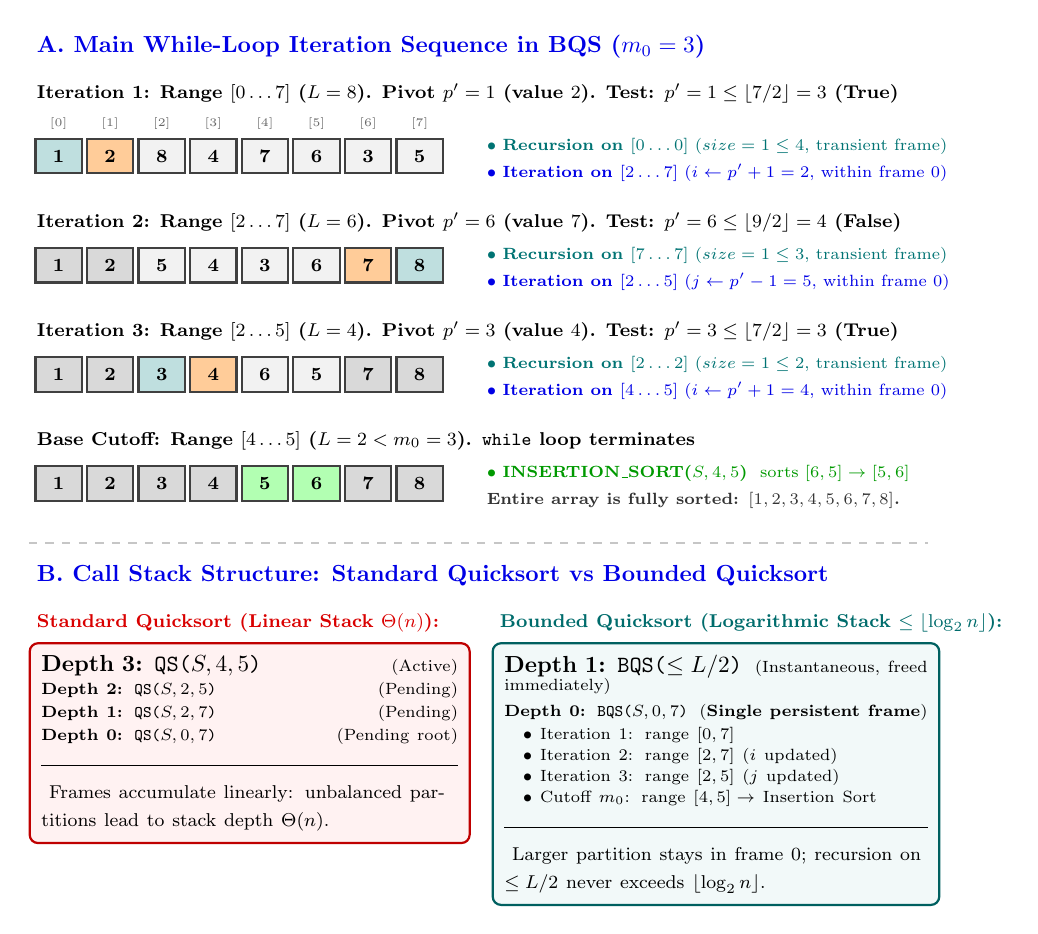
\begin{tikzpicture}[
    scale=0.84,
    every node/.style={transform shape},
    ptr/.style={-{Stealth[scale=1.0]}, very thick, draw=blue!85!black},
    ptrLbl/.style={font=\scriptsize\bfseries, text=blue!90!black},
    cell/.style={rectangle, draw=black!75, thick, minimum width=0.70cm, minimum height=0.52cm, font=\footnotesize\bfseries, align=center},
    frameBox/.style={rectangle, draw=teal!75!black, fill=teal!5, rounded corners=3pt, thick, inner sep=5pt},
    classicBox/.style={rectangle, draw=red!75!black, fill=red!5, rounded corners=3pt, thick, inner sep=5pt}
  ]
    % --- PART A: BQS Execution Trace ---
    \node[anchor=west, font=\normalsize\bfseries, text=blue!90!black] at (0, 8.4) {\textbf{A. Main While-Loop Iteration Sequence in BQS} ($m_0=3$)};

    % Iteration 1
    \node[anchor=west, font=\footnotesize\bfseries] at (0, 7.7) {Iteration 1: Range $[0 \dots 7]$ ($L=8$). Pivot $p'=1$ (value $2$). Test: $p'=1 \le \lfloor 7/2 \rfloor = 3$ (True)};
    \foreach \val/\col/\idx/\c in {1/teal!25/0/0, 2/orange!40/1/1, 8/gray!10/2/2, 4/gray!10/3/3, 7/gray!10/4/4, 6/gray!10/5/5, 3/gray!10/6/6, 5/gray!10/7/7} {
      \node[cell, fill=\col] at (0.45 + \c*0.78, 6.75) {\val};
      \node[above=0.5pt, font=\tiny\color{black!60}] at (0.45 + \c*0.78, 7.01) {[\idx]};
    }
    \node[anchor=west, font=\scriptsize, text=teal!90!black] at (6.8, 6.9) {$\bullet$ \textbf{Recursion on $[0 \dots 0]$} ($\text{size}=1 \le 4$, transient frame)};
    \node[anchor=west, font=\scriptsize, text=blue!90!black] at (6.8, 6.5) {$\bullet$ \textbf{Iteration on $[2 \dots 7]$} ($i \leftarrow p'+1=2$, within frame 0)};

    % Iteration 2
    \node[anchor=west, font=\footnotesize\bfseries] at (0, 5.75) {Iteration 2: Range $[2 \dots 7]$ ($L=6$). Pivot $p'=6$ (value $7$). Test: $p'=6 \le \lfloor 9/2 \rfloor = 4$ (False)};
    \foreach \val/\col/\c in {1/black!15/0, 2/black!15/1, 5/gray!10/2, 4/gray!10/3, 3/gray!10/4, 6/gray!10/5, 7/orange!40/6, 8/teal!25/7} {
      \node[cell, fill=\col] at (0.45 + \c*0.78, 5.1) {\val};
    }
    \node[anchor=west, font=\scriptsize, text=teal!90!black] at (6.8, 5.25) {$\bullet$ \textbf{Recursion on $[7 \dots 7]$} ($\text{size}=1 \le 3$, transient frame)};
    \node[anchor=west, font=\scriptsize, text=blue!90!black] at (6.8, 4.85) {$\bullet$ \textbf{Iteration on $[2 \dots 5]$} ($j \leftarrow p'-1=5$, within frame 0)};

    % Iteration 3
    \node[anchor=west, font=\footnotesize\bfseries] at (0, 4.1) {Iteration 3: Range $[2 \dots 5]$ ($L=4$). Pivot $p'=3$ (value $4$). Test: $p'=3 \le \lfloor 7/2 \rfloor = 3$ (True)};
    \foreach \val/\col/\c in {1/black!15/0, 2/black!15/1, 3/teal!25/2, 4/orange!40/3, 6/gray!10/4, 5/gray!10/5, 7/black!15/6, 8/black!15/7} {
      \node[cell, fill=\col] at (0.45 + \c*0.78, 3.45) {\val};
    }
    \node[anchor=west, font=\scriptsize, text=teal!90!black] at (6.8, 3.6) {$\bullet$ \textbf{Recursion on $[2 \dots 2]$} ($\text{size}=1 \le 2$, transient frame)};
    \node[anchor=west, font=\scriptsize, text=blue!90!black] at (6.8, 3.2) {$\bullet$ \textbf{Iteration on $[4 \dots 5]$} ($i \leftarrow p'+1=4$, within frame 0)};

    % Iteration 4 (Cutoff)
    \node[anchor=west, font=\footnotesize\bfseries] at (0, 2.45) {Base Cutoff: Range $[4 \dots 5]$ ($L=2 < m_0=3$). \texttt{while} loop terminates};
    \foreach \val/\col/\c in {1/black!15/0, 2/black!15/1, 3/black!15/2, 4/black!15/3, 5/green!30/4, 6/green!30/5, 7/black!15/6, 8/black!15/7} {
      \node[cell, fill=\col] at (0.45 + \c*0.78, 1.8) {\val};
    }
    \node[anchor=west, font=\scriptsize, text=green!60!black] at (6.8, 1.95) {$\bullet$ \textbf{INSERTION\_SORT($S, 4, 5$)} $\implies$ sorts $[6, 5] \to [5, 6]$};
    \node[anchor=west, font=\scriptsize\bfseries, text=black!80] at (6.8, 1.55) {Entire array is fully sorted: $[1, 2, 3, 4, 5, 6, 7, 8]$.};

    % Horizontal separator
    \draw[thick, dashed, draw=gray!45] (0, 0.9) -- (13.6, 0.9);

    % --- PART B: Call Stack Comparison ---
    \node[anchor=west, font=\normalsize\bfseries, text=blue!90!black] at (0, 0.4) {\textbf{B. Call Stack Structure: Standard Quicksort vs Bounded Quicksort}};

    % Stack Classic
    \node[anchor=west, font=\footnotesize\bfseries, text=red!85!black] at (0, -0.3) {Standard Quicksort (Linear Stack $\Theta(n)$):};
    \node[classicBox, anchor=north west, text width=6.3cm, align=left] at (0, -0.6) {
      \textbf{Depth 3:} \texttt{QS($S, 4, 5$)} \hfill \scriptsize (Active)\\[2pt]
      \textbf{Depth 2:} \texttt{QS($S, 2, 5$)} \hfill \scriptsize (Pending)\\[2pt]
      \textbf{Depth 1:} \texttt{QS($S, 2, 7$)} \hfill \scriptsize (Pending)\\[2pt]
      \textbf{Depth 0:} \texttt{QS($S, 0, 7$)} \hfill \scriptsize (Pending root)\\[3pt]
      \rule{\linewidth}{0.4pt}\\[2pt]
      \footnotesize $\implies$ Frames accumulate linearly: unbalanced partitions lead to stack depth $\Theta(n)$.
    };

    % Stack BQS
    \node[anchor=west, font=\footnotesize\bfseries, text=teal!85!black] at (7.0, -0.3) {Bounded Quicksort (Logarithmic Stack $\le \lfloor\log_2 n\rfloor$):};
    \node[frameBox, anchor=north west, text width=6.4cm, align=left] at (7.0, -0.6) {
      \textbf{Depth 1:} \texttt{BQS($\le L/2$)} \hfill \scriptsize (Instantaneous, freed immediately)\\[3pt]
      \textbf{Depth 0:} \texttt{BQS($S, 0, 7$)} \hfill \scriptsize (\textbf{Single persistent frame})\\[2pt]
      \quad $\bullet$ Iteration 1: range $[0, 7]$\\[1pt]
      \quad $\bullet$ Iteration 2: range $[2, 7]$ ($i$ updated)\\[1pt]
      \quad $\bullet$ Iteration 3: range $[2, 5]$ ($j$ updated)\\[1pt]
      \quad $\bullet$ Cutoff $m_0$: range $[4, 5] \to$ Insertion Sort\\[3pt]
      \rule{\linewidth}{0.4pt}\\[2pt]
      \footnotesize $\implies$ Larger partition stays in frame 0; recursion on $\le L/2$ never exceeds $\lfloor\log_2 n\rfloor$.
    };

  \end{tikzpicture}
  \caption{Execution trace of Bounded Quicksort (BQS) with threshold $m_0=3$ and call stack memory comparison. (\textbf{A}) At each iteration, the larger partition is processed within the same stack frame by updating $i$ or $j$, while only the halved partition ($\le L/2$) triggers a short-lived recursive call. (\textbf{B}) Standard Quicksort accumulates call frames linearly; BQS strictly guarantees logarithmic stack depth.}
  \label{fig:bqs-trace-and-stack}
\end{figure}

In \autoref{tab:bqs-execution-trace}, the step-by-step iteration sequence is detailed, highlighting the smaller-partition test, the tail recursion elimination update, and the instantaneous maximum stack depth.

\begin{table}[H]
  \centering
  \noindent\makebox[\textwidth][c]{%
  \footnotesize
  \setlength{\tabcolsep}{4.5pt}
  \begin{tabular}{c c c c l c c}
    \toprule
    \textbf{Step} & $\boldsymbol{[i, j]}$ & $\boldsymbol{L}$ & \textbf{Pivot Test} & \textbf{Action (Recursion \& Iteration)} & \textbf{Array State} & \textbf{Stack} \\
    \midrule
    Init & $[0, 7]$ & 8 & -- & Root frame $\text{BQS}(S, 0, 7)$ & $[7, 2, 8, 4, 1, 6, 3, 5]$ & 0 \\
    \addlinespace[3pt]
    1 & $[0, 7]$ & 8 & $p'=1 \le 3$ & 
    \begin{tabular}{@{}ll@{}}
      \textbf{Rec:}  & $[0, 0]$ ($\text{size} \le 4$, instant return) \\
      \textbf{Iter:} & $i \leftarrow 2$ on $[2, 7]$ (same frame)
    \end{tabular} & $[1 \mid \mathbf{2} \mid 8, 4, 7, 6, 3, 5]$ & 1 \\
    \addlinespace[3pt]
    2 & $[2, 7]$ & 6 & $p'=6 > 4$ & 
    \begin{tabular}{@{}ll@{}}
      \textbf{Rec:}  & $[7, 7]$ ($\text{size} \le 3$, instant return) \\
      \textbf{Iter:} & $j \leftarrow 5$ on $[2, 5]$ (same frame)
    \end{tabular} & $[1, 2 \mid 5, 4, 3, 6 \mid \mathbf{7} \mid 8]$ & 1 \\
    \addlinespace[3pt]
    3 & $[2, 5]$ & 4 & $p'=3 \le 3$ & 
    \begin{tabular}{@{}ll@{}}
      \textbf{Rec:}  & $[2, 2]$ ($\text{size} \le 2$, instant return) \\
      \textbf{Iter:} & $i \leftarrow 4$ on $[4, 5]$ (same frame)
    \end{tabular} & $[1, 2 \mid 3 \mid \mathbf{4} \mid 6, 5 \mid 7 \mid 8]$ & 1 \\
    \midrule
    Cutoff & $[4, 5]$ & 2 & $L < m_0$ & 
    \begin{tabular}{@{}ll@{}}
      \textbf{Exit:} & Exit \texttt{while} loop \\
      \textbf{Sort:} & Insertion Sort on $[4, 5]$
    \end{tabular} & $[1, 2, 3, 4, \mathbf{5, 6}, 7, 8]$ & 0 \\
    \bottomrule
  \end{tabular}%
  }
  \caption{Step-by-step trace of Bounded Quicksort (BQS) with cutoff threshold $m_0=3$. In each iteration, the subproblem of size $\le L/2$ is resolved with a bounded recursive call, while the larger subproblem is processed iteratively within the current frame, bounding stack depth to $\le 1$ in this trace ($\le \lfloor \log_2 n \rfloor$ in general).}
  \label{tab:bqs-execution-trace}
\end{table}

\FloatBarrier

\subsection{Rigorous Analysis of the \texorpdfstring{$\Theta(\log_2 n)$}{Theta(log n)} Extra Space Bound}
\label{subsec:bqs-space-analysis}

The cornerstone of BQS lies in its absolute mathematical guarantee on memory consumption:

\begin{theorem}[Auxiliary Space Guarantee of Bounded Quicksort]
\label{thm:bqs-space-guarantee}
For any input of size $n$, Bounded Quicksort consumes an auxiliary call stack space strictly bounded by:
\begin{equation}
  \text{Auxiliary Space} = \Theta(\log_2 n).
\end{equation}
The maximum stack depth never exceeds $\lfloor \log_2 n \rfloor$ under any worst-case scenario.
\end{theorem}

\begin{proof}
Let $L = j - i + 1$ denote the length of the active subarray at the entry of a BQS call. Upon partitioning around index $p'$, the algorithm inspects the lengths of the two subranges:
\begin{itemize}
  \item The left subrange has length $L_{\text{left}} = (p' - 1) - i + 1 = p' - i$.
  \item The right subrange has length $L_{\text{right}} = j - (p' + 1) + 1 = j - p'$.
\end{itemize}
The condition $p' \le \lfloor \frac{i + j}{2} \rfloor$ implies:
\begin{equation}
  p' - i \le \frac{j - i}{2} < \frac{L}{2}.
\end{equation}
Consequently, when this condition holds, recursion is invoked exclusively on the left partition, whose size is strictly bounded by:
\begin{equation}
  L_{\text{recursive}} \le \left\lfloor \frac{L}{2} \right\rfloor.
\end{equation}
Conversely, when $p' > \lfloor \frac{i + j}{2} \rfloor$, the right subrange satisfies $j - p' < \frac{L}{2}$, and the recursive call is invoked on the right partition, fulfilling the exact same inequality.

The remaining subproblem has size $L_{\text{iterative}} \ge \frac{L}{2}$, but \textbf{does not spawn any recursive call}: the algorithm simply mutates $i \leftarrow p' + 1$ or $j \leftarrow p' - 1$ and loops within the existing activation frame without allocating any new stack space.

Therefore, the input size passed to any subsequent stack frame decreases by at least a factor of $2$ relative to its parent frame:
\begin{equation}
  L^{(k)} \le \frac{n}{2^k},
\end{equation}
where $k$ denotes the current stack depth. The recursion can continue at most while $L^{(k)} \ge m_0 \ge 1$:
\begin{equation}
  \frac{n}{2^k} \ge 1 \implies 2^k \le n \implies k \le \lfloor \log_2 n \rfloor.
\end{equation}
Since each activation record requires constant memory $\mathcal{O}(1)$, the total auxiliary stack space is strictly bounded by:
\begin{equation}
  \text{Extra Space} = \mathcal{O}(1) \cdot \lfloor \log_2 n \rfloor = \Theta(\log_2 n).
\end{equation}
\end{proof}

\subsection{Hybrid Optimization with Insertion Sort Cutoff}
\label{subsec:bqs-cutoff-insertion-sort}

Introducing a threshold $m_0 \in [16, 32]$ for handing off small subproblems to \textit{Insertion Sort} directly leverages hardware caching characteristics and execution profile:

\begin{itemize}
  \item \textbf{Elimination of Recursive Overhead:} When subarray size drops below $m_0$, the overhead of function call frames, parameter passing, and partition pointer management surpasses the computational cost of direct comparisons.
  \item \textbf{Low Constant Factors of Insertion Sort:} \textit{Insertion Sort} has exceptionally low constant factors: it requires no extra heap or stack space, runs tight inner loops, and easily undergoes compiler vectorization and loop unrolling.
  \item \textbf{Optimal L1 Cache Locality:} A block of $16 \div 32$ items requires approximately $128 \div 256$ bytes (for 64-bit keys), fitting completely within one or two 64-byte L1 cache lines. All comparisons and shifts occur without generating any cache misses.
  \item \textbf{Nearly Sorted Behavior:} Because Quicksort's macro-partitions have already placed elements near their final positions, small subarrays are almost sorted. On nearly sorted inputs, Insertion Sort operates in linear time $\mathcal{O}(n)$ rather than quadratic time.
\end{itemize}

In conclusion, Bounded Quicksort represents an ideal synthesis of mathematical rigor and algorithm engineering, guaranteeing optimal expected time complexity $\mathcal{O}(n \log_2 n)$, absolute immunity to \textit{Stack Overflow} via $\Theta(\log_2 n)$ auxiliary space, and exceptional empirical throughput on modern computer architectures.
